\section{\secState{D}Hybrid Automaton}\label{s:HybridAutomaton}
    \noindent First the notion of  \emph{hybrid} automaton  \cite{lazar2006model,borrelli2006mpc,daws1996tool} needs to be introduced:

    \begin{definition}{Hybrid automaton} (\ref{eq:hybridAutomaton}) is given as structure:
        \begin{equation}\label{eq:hybridAutomaton}
        \begin{aligned}
            HybridAutomaton(&Automaton States, SystemState, VectorField, \\
                            &DiscreteTransition,ResetMap)
        \end{aligned}
        \end{equation}
    
        \noindent \emph{Automaton States} is given as set of discrete states, for every time $time\in Domain$ hybrid automaton stays in exactly one of \emph{states}.
    
        \emph{System State}, is given in domain $x\in\R^n,n\in\N^+$, representing the trajectory evolution.
        
        emph{Vector Field} (\ref{eq:vectorField}) is bounded to single $Automaton State$ and represents local System State evolution, when given automaton State is Active.
        
        \begin{equation}\label{eq:vectorField}
            VectorField: Automaton StateState\times SystemState \to SystemState
        \end{equation}
        
        \noindent\emph{DiscreteTransition} (eq. \ref{eq:discreteTransition}) indicates changes of states in automaton, the changes are triggered by satisfying specific condition given by Automaton State and System State. 
        
        \begin{equation}\label{eq:discreteTransition}
            DiscreteTransition:Automaton State\times SystemState \to Automaton State
        \end{equation}
        
        \noindent \emph{ResetMap} (eq. \ref{eq:resetMap}) defines changes of State to some default value, this change is triggered by specific automaton State and System State.
        
        \begin{equation}\label{eq:resetMap}
            ResetMap:State\times SystemState \to SystemState
        \end{equation}
    
    \end{definition}

\paragraph{Hybrid Automaton Example:} An example of \emph{hybrid automaton} is given in (fig. \ref{fig:hybridAtomatonExample}). The automaton is used to control \emph{UAS system} to perform simple level up (increase altitude) maneuver \cite{casau2011uav}. The automaton has three discrete states representing \emph{hover}, \emph{transition}, and, \emph{level} portion of the maneuver.

\begin{figure}[H]
    \centering
    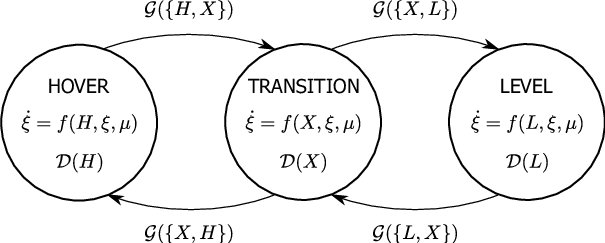
\includegraphics[width=0.60\linewidth]{\FIGDIR/BC001HybridAutomatonExample} 
    \caption{Example: The hybrid automaton example for UAS manuever \cite{casau2011uav}.}
    \label{fig:hybridAtomatonExample}
\end{figure}
